
\section{Evaluation}
\label{sec:eval}



% \begin{figure}
% 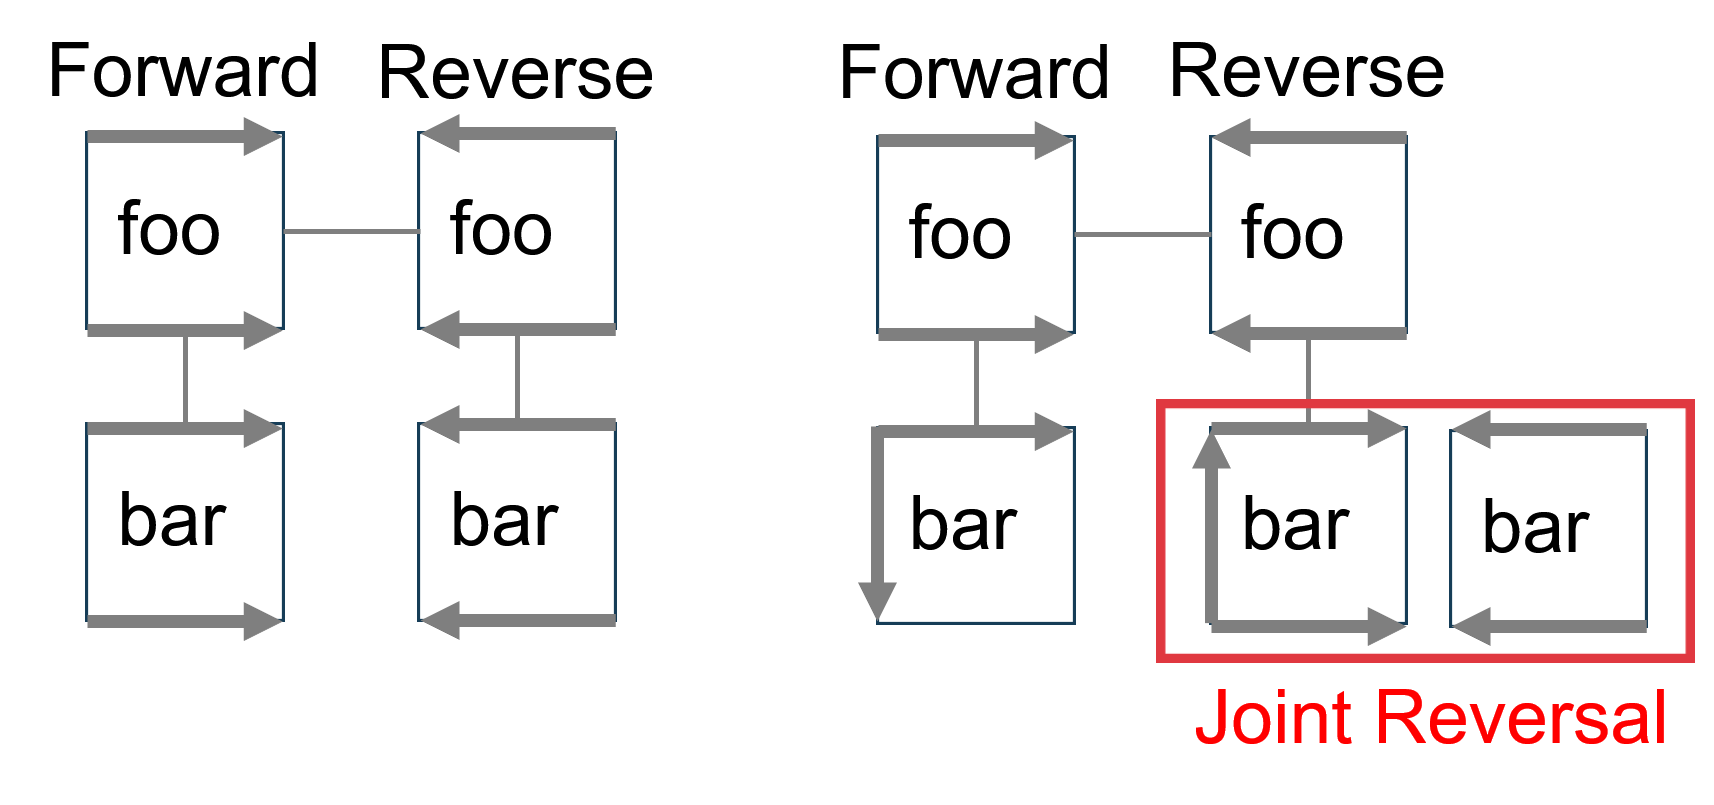
\includegraphics[width=\linewidth]{figures/joint.png}
% \caption{Reversal modes for function calls: Split reversal (left), joint reversal (right)}
% \label{fig:reversalmodes}
% \end{figure}

% % Marked as a potential for cutting text
% GPU kernels are implemented as function calls in a larger applications computer program, with the kernels being the leafs of the call tree. There are two ways of reversing a computer program for the gradient evaluation shown in \reffig{fig:reversalmodes}. {\it Split reversal} splits the entire computer program into the forward and reverse pass, where every function is first computing the primal intermediate values and storing them on a stack (double forward arrow) while restoring them (double reverse arrow) in the reverse pass. {\it Joint reversal} of a function recomputes the primal values by restoring only the inputs (up arrow) stored in the forward pass (down arrow) and then does a reverse pass in the same function call. Joint reversal trades memory storage for recomputation cost and is the obvious choice for GPU kernels with restricted memory availability; the joint reversed program uses less memory. In the following analysis we evaluate the joint reversed implementation (red) of GPU kernels.

% Rewrite of evaluation paragraph
\change{We evaluate our approach on five established GPU-based HPC proxy applications:}
\begin{itemize}
    \item CUDA-based RSBench~\cite{RSBench} and XSBench~\cite{XSBench}, two implementations of Monte Carlo neutron transport algorithms
    \item An extended version of the CUDA lattice-Boltzmann method (LBM) solver from the Parboil benchmark suite~\cite{stratton2012parboil}, with applications in computational fluid dynamics
    \item CUDA-based Livermore Unstructured Lagrangian Explicit Shock Hydrodynamics (LULESH) code~\cite{LULESH2:changes}, a proxy application for computational fluid dynamics solvers% on Exascale systems
    \item A discontinuous-Galerkin (DG) volume integral\footnote{\url{https://github.com/lcw/Heptapus.jl}}\cite{dg_wilcox} kernel as used in the pure Julia~\cite{bezanson2017julia} climate code ClimateMachine.jl\footnote{\url{https://github.com/CliMA/ClimateMachine.jl/}}~\cite{clima2017} and implemented for both CUDA and AMD GPUs
\end{itemize}


\subsection{Setup}

For each application, we time just the evaluation of the code being differentiated, excluding time taken for device memory initialization and transfer or other calling code. \change{For CUDA kernels, we explicitly increase the size of the device heap to 1 GB. RSBench, XSBench, and the CUDA.jl version of DG were evaluated on an NVIDIA 2080 Super. LBM was evaluated on an NVIDIA V100. LULESH was evaluated on an NVIDIA RTX A6000. The AMDGPU.jl version of DG was evaluated on an AMD Vega 64. Benchmarks were tested with LLVM main at commit \texttt{8dab25954b0acb53731c4aa73e9a7f4f98263030}, Julia 1.6, and Enzyme at commit \texttt{ec75831a8cb0}. The benchmark suite is available at \url{https://github.com/wsmoses/Enzyme-GPU-Tests}.}

All benchmarks were evaluated a minimum of five times, taking the geometric mean as the final result. \change{For each benchmark we evaluated the original kernel and the combined forward/reverse pass generated by Enzyme (Figure \ref{fig:app_performance}); the combined forward and reverse pass with various optimizations described in Section \ref{sec:opt} disabled (Figure \ref{fig:effect_of_optimisations}); the compile times of the benchmarks (Figure \ref{fig:comptime}); and the scalability of the gradients compared to the original code (Figures \ref{fig:relweak} and \ref{fig:probinc}).}


\begin{figure}
    \centering
    \includestandalone[width=.45\textwidth]{figures/Candlesticks}
    \caption{AD overhead of the benchmark applications, as compared with a single evaluation of the forward pass. \change{An overhead of $N$ can be read as saying that collecting the gradients of all inputs (as well as running the original code) is equivalent to running the original code $N$ times.}}
    \label{fig:app_performance}
\end{figure}

\begin{figure}
    \centering
\begin{minted}[fontsize=\small]{cuda}
void kern(float* src, float* dst) {
    streamCollide<<<...>>>(src, dst);
}

void lbm(int nTimeSteps, float* src, float* dst) {
    for (unsigned int i=0; i<nTimeSteps/2; i++) {
        kern(src, dst);
        kern(dst, src);
    }
}
\end{minted}
    \caption{\change{Simplified version of the computation within LBM. The \texttt{kern} function calls a GPU kernel that iterates the simulation one timestep forward in time, storing the result in \texttt{dst}. The \texttt{lbm} CPU function calls the GPU kernel until all iterations have completed. The iteration must happen outside the kernel to ensure that all threads from one timestep have completed prior to performing another timestep.}}
    \label{fig:lbm}
\end{figure}

\change{With the exception of the LBM benchmark (see below), modifying a benchmark to enable differentiation simply required allocating and initializing shadow arrays (to store the output gradients), and creating a kernel which calls \texttt{\_\_enzyme\_autodiff} on the kernel to be differentiated, as demonstrated in Figure \ref{fig:exdiff}.}

\change{The correctness of the generated gradients was verified by comparing with numeric differentiation. Since our benchmarks have too many parameters to use numeric differentiation effectively, only a few inputs per benchmarks were tested. }

\subsection{Benchmark Descriptions}

\paragraph{\textbf{RSBench and XSBench}}
RSBench and XSBench are U.S. Department of Energy proxy applications that represent the core computation of Monte Carlo simulations within particle transport algorithms such as in OpenMC~\cite{romano2013openmc}. The majority of the runtime of XSBench is spent in memory operations with a semi-random access pattern. By calculating neutron cross-sections with the multipole method, RSBench trades off several magnitudes of memory in exchange for a significant amount of computation to unpack the data. Together, RSBench and XSBench allow us to differentiate both compute-bound and memory-bound applications, respectively.



\begin{figure*}
    \centering
\begin{tabular}{c|c}
\textbf{(a)}&\textbf{(b)}\vspace*{-3mm}
\\
\begin{minipage}[T]{0.48\linewidth}
\begin{minted}[fontsize=\small]{cuda}
// CPU Code
void aug_kern(float* src, float *dsrc,
              float* dst, float* ddst) {
  void* tape = Allocator.allocate(...);
  aug_streamCollide<<<...>>>(src, dsrc, dst, ddst, tape);
}
void grad_kern(float* src, float *dsrc,
               float* dst, float* ddst, void* tape) {
  grad_streamCollide<<<...>>>(src, dsrc, dst, ddst, tape);
  Allocator.free(tape);
}
__attribute__((enzyme(aug_kern, grad_kern)))
void kern(float* src, float* dst);

void grad_lbm(int nTimeSteps, float* src, float* dsrc,
                              float* dst, float* ddst) {
  __enzyme_autodiff(lbm, nTimeSteps, src, dsrc, dst, ddst);
}
\end{minted}
\end{minipage}&\begin{minipage}[T]{0.48\linewidth}
\begin{minted}[fontsize=\small, escapeinside=||]{cuda}
// GPU Code
__global__
void aug_streamCollide(float* src, float* dsrc,
                       float* dst, float* ddst, void** tape) {
  size_t idx = threadIdx.x + ...;
  tape[idx] = __enzyme_augmentfwd(streamCollide, src, dsrc,
                                    dst, ddst);
}

__global__
void grad_streamCollide(float* src, float* dsrc,
                        float* dst, float* ddst, void** tape) {
  size_t idx = threadIdx.x + ...;
  __enzyme_reverse(streamCollide, src, dsrc,
                   dst, ddst, tape[idx]);
}

|\;|
\end{minted}
\end{minipage}
\end{tabular}
    \caption{\change{Differentiation of the combined CPU+GPU computation in LBM. The code in (a) represents host code, which differentiates the overall function \texttt{lbm}, defined in Figure \ref{fig:lbm}. The \texttt{kern} function is annotated with custom forward and reverse passes \texttt{aug\_kern} and \texttt{grad\_kern}. These functions allocate a tape and call the \texttt{aug\_streamCollide} and \texttt{grad\_streamCollide} kernels, which are generated by Enzyme in (b).}}
    \label{fig:lbm_ad}
\end{figure*}

\paragraph{\textbf{Lattice Boltzmann Method (LBM)}}
LBM is a particle-based fluid dynamics simulation method. It works by modeling fluid density on a lattice (grid) and in each time step performing a streaming step (allowing fluid to flow into adjacent grid cells) and a collision step (which models the interaction of fluids flowing into a particular cell from neighboring cells). This so-called stream-collide sequence is responsible for the majority of the computational cost of typical LBM solvers and is implemented in the CUDA version of Parboil LBM in a method called \texttt{performStreamCollide\_kernel}. \change{ CPU driver code calls this kernel in a loop to advance the simulation by several timesteps, as shown in Figure ~\ref{fig:lbm}. }

\change{
Unlike the other benchmarks tested, where the entire function being differentiated was on the GPU, differentiating LBM requires the differentiation of heterogeneous programs. Since LLVM does not yet support modules which contain both CPU and GPU code, we perform differentiation in two steps. First, we use Enzyme to generate an augmented forward and reverse pass for the GPU kernel. The forward pass is equivalent to the original function, saving any data that is required for the reverse pass and may be overwritten. The forward and reverse pass of the GPU kernels can then be imported into the CPU code by using Enzyme's support for custom derivatives. The heterogeneous AD setup is demonstrated in Figure ~\ref{fig:lbm_ad}. Note that while we demonstrate this shim layer for clarity, in practice this can be simplified for end users through the use of advanced compiler transformations or macros.}%
%
% There are other versions implemented e.g. for CPUs or in OpenCL, which we did not consider here.

\paragraph{\textbf{LULESH}}
LULESH~\cite{LULESH2:changes} is an unstructured explicit shock hydrodynamics solver, which was initially introduced as a proxy application for computational fluid dynamics on high-performance computing systems and has since been employed as a proxy application for complex fluid dynamics codes. % on \change{next-generation} systems. %
\change{LULESH emulates complex hydrodynamic solvers by splitting the computational domain into volumetric elements on an unstructured mesh. This allows LULESH to mimic the complex data movement characteristics of unstructured data structures.}
% AD variables were initialized through the definition in the header file and then passed down through the domain initialization into the individual kernels in the \textit{LagrangeLeapFrog} step.
All measurements were analyzed with  NVIDIA NSight Compute to discern the individual measurements of the gradient \textit{ApplyMaterialPropertiesAndUpdateVolume} kernel from the general application runtime.

\begin{figure*}
    \centering
    \includestandalone[width=\textwidth]{figures/stacked2}
    \caption{\change{Overhead of selectively disabling AD and GPU-specific optimizations described in Section \ref{sec:opt}. OOM indicates running out of memory or an indefinite runtime. Each dot represents the overhead of AD compared to the forward pass alone.}}
    \label{fig:effect_of_optimisations}
\end{figure*}

\paragraph{\textbf{Discontinuous Galerkin (DG)}}
The  discontinuous-\-Galerkin  volume integral\cite{dg_wilcox} kernel is part of a fluid dynamics simulation model. It is written in Julia, and we use \texttt{CUDA.jl}~\cite{besard2018juliagpu} and \texttt{AMDGPU.jl}~\cite{AMDGPU2021} in combination with Enzyme.jl~\cite{enzymeNeurips} to synthesize and execute the kernel and its derivative. The code features GPU-specific features, such as shared memory, and is memory bound. We modified the original code to use noncoherent memory loads in the case of \texttt{CUDA.jl} and constant memory loads in the case of \texttt{AMDGPU.jl}.

\subsection{Results}

The original Enzyme paper \cite{enzymeNeurips} demonstrated that by embedding AD within the compiler, one can perform AD after optimization which is on average $4.2\times$ faster than AD before optimization.
\change{Since prior tools perform AD at a source level, they must perform AD prior to any compiler optimizations.}
Although there exist no tools that we can compare against that perform reverse-mode AD on GPU kernels, we attempted to perform a similar ablation analysis here to see what a tool not implemented within a compiler might be able to achieve, if one were to be written. \change{ Without applying standard LLVM optimizations prior to AD, RSBench and XSBench take an indefinite amount of time to run. LULESH has an overhead of $2979.1\times$ without preprocessing optimizations. LBM is able to be differentiated without preprocessing optimizations for two iterations, but exhausts GPU memory on anything larger (scaling tests use 50-600 iterations). In order to legalize Julia code for the GPU (such as the ROCm and CUDA DG codes), it is necessary to run the LLVM optimization pipeline, along with Julia's custom optimization passes. }
We therefore conclude that the ability to run optimizations alongside AD is in fact a precondition of successful reverse-mode AD of general GPU programs.

Overall, the combined forward and gradient generated by Enzyme have a reasonable overhead when compared with that  of the forward pass (Figure~\ref{fig:app_performance}). RSBench and XSBench have a $3-4\times$ overhead due to the need to cache intermediate computations from the forward pass. Similarly, LBM must cache the current state variables every iteration leading to an overhead of $6.3\times$. The kernel evaluated in LULESH does not need to cache additional values, and as a result the \change{$2.01\times$} overhead is spent performing the corresponding gradient computations. The DG benchmark has a $5.4\times$ overhead when run on AMD, primarily from the additional computation, whereas it has a $18\times$ overhead on CUDA as it quickly exhausts the amount of available registers and the CUDA assembler decides to spill a large number of registers into global memory.

\paragraph{\textbf{AD and GPU-Specific Optimizations}}
\change{
To evaluate the effectiveness of the optimizations described in Section \ref{sec:opt}, we evaluated all benchmarks with several AD and GPU-specific optimizations being successively disabled. Not all benchmarks benefit from the same optimizations, and the order in which compiler optimizations are applied can dramatically impact performance~\cite{autophase}. For each benchmark, we visualize a path through the exponentially large optimization space that attempts to enable each optimization when it will have the largest impact on performance. The results of this analysis are shown in Figure \ref{fig:effect_of_optimisations}. An end user trying to maximize their performance wouldn't explore all optimization combinations/paths, instead simply enabling all optimizations. As disabling optimizations quickly blows up the runtime of the program, the ablation analysis of benchmarks was run at a smaller test size to ensure the computation completed in a reasonable time where necessary. 

For the ROCm DG kernel, an unrolling optimization was necessary to allow Enzyme to create the gradient without caching any additional values. Without unrolling, the GPU was unable to allocate sufficient device memory to succeed.

For the CUDA DG kernel, simply applying the standard Julia+LLVM optimization pipeline enabled the gradient to run, though at a $1378.3\times$ overhead. Running an optimization that coalesced multiple allocations into a single \texttt{malloc} call reduced this runtime to $116.6\times$. Like in the ROCm case, applying unrolling eliminates any need to cache values, reducing the overhead to $17.8\times$.

For ablation analysis, we ran the LBM kernel for 150 iterations. The use of an efficient CPU to GPU calling convention for caching values was necessary for the gradient to run on a problem of this size. Applying the improved recompute vs cache heuristic allowed Enzyme to detect that it could cache a double which representing a sum, rather than the individual of overwritten values. This analysis reduced the size of the cache from $80$ bytes per thread to $20$ bytes per thread. As a result, the AD overhead was reduced from $19.87\times$ to $8.7\times$. Finally, using a LIFO allocator rather than \texttt{cudaMalloc} to allocate cache memory brought the AD overhead down to $6.4\times$.

For ablation analysis, LULESH was run on a computational domain size of $90^{3}$. Applying just LLVM optimizations prior to AD brought the LULESH gradient overhead down to $2.4\times$ from $2979.1\times$. As the LULESH kernel was particularly branch heavy, enabling speculative execution of $\phi$ predecessors when recomputing values in the reverse pass reduced the AD overhead down to $2.01\times$.

Running RSBench on a problem size of 10,200, LLVM optimizations alone resulted in an overhead of $6374\times$. By applying additional inlining, this overhead was reduced to $9.5\times$ as LLVM could optimize between functions, enabling Enzyme to eliminate redundant values being cached, as well as use a more efficient intraprocedural caching infrastructure. Enabling the loop invariant cache and equivalent load cache optimizations reduced the overhead down to $4.7\times$.

Running XSBench on a problem size of 17,000,000 with LLVM optimizations, the overhead was $25.9\times$. Allowing Enzyme to avoid caching loop bounds when it can prove that all its instructions are inactive, drops the overhead to $16.3\times$. Performing PHI restructuring reduces the overhead to $9.5\times$. Passing the mode of simulation through a C++ template eliminates code generation of helper routines from different simulation modes and reduces the overhead to $3.2\times$. This leads to fewer branches in the forward pass and allows Enzyme to avoid analogous branches in the reverse pass.
}

% \begin{figure}
%     \centering
%     \begin{tabular}{l|r}
%          Test & Overhead \\\hline
%          Forward & 1 \\
%          AD, Optimized & 4.4 \\
%          - CacheLICM & 343.7 \\
%          - Recompute Heuristic & 1275.6 \\
%          - Inlining & 6372.2 \\
%          - PreOptimization & OOM \\
%     \end{tabular}
%     % \includestandalone[width=.45\textwidth]{figures/EffectOfOptimizations}
%     \caption{Overhead of progressively disabling AD and GPU-specific optimizations described in Section \ref{sec:opt} when evaluated on RSBench. OOM indicates that the test ran out of memory.}
%     \label{fig:effect_of_optimisations}
% \end{figure}


% \begin{figure}
%     \centering
%     \begin{tabular}{l|r}
%          Test & Overhead \\\hline
%          Forward & 1 \\
%          AD, Optimized & 3.16 \\
%          - Templating & 9.61 \\
%          - PHI Recompute & 14.47 \\
%          - Alias Analysis & 47.40 \\
%          - Recompute Heuristic & 95.75 \\
%          - PreOptimization & OOM \\
%     \end{tabular}
%     % \includestandalone[width=.45\textwidth]{figures/EffectOfOptimizations}
%     \caption{Overhead of selectively disabling AD and GPU-specific optimizations described in Section \ref{sec:opt} when evaluated on XSBench. OOM indicates that the test ran out of memory.}
%     \label{fig:effect_of_optimisations}
% \end{figure}



% \begin{figure}
%     \centering
%     \begin{tabular}{l|r}
%          Test & Overhead \\\hline
%          Forward & 1 \\
%          AD, Optimized & 6.39 \\
%          - Custom Allocator & 8.74 \\
%          - Recompute Heuristic & 19.87 \\
%          - Inline Cache ABI & OOM \\
%          - PreOptimization & OOM \\
%     \end{tabular}
%     % \includestandalone[width=.45\textwidth]{figures/EffectOfOptimizations}
%     \caption{Overhead of selectively disabling AD and GPU-specific optimizations described in Section \ref{sec:opt} when evaluated on LBM with 150 iterations. OOM indicates that the test ran out of memory.}
%     \label{fig:effect_of_optimisations}
% \end{figure}


% \begin{figure}
%     \centering
%     \begin{tabular}{l|r}
%          Test & Overhead \\\hline
%          Forward & 1 \\
%          AD, Optimized & 17.85 \\
%          - Unrolling & 116.63 \\
%          - Malloc Coalesing & 1378.32 \\
%     \end{tabular}
%     % \includestandalone[width=.45\textwidth]{figures/EffectOfOptimizations}
%     \caption{Overhead of selectively disabling AD and GPU-specific optimizations described in Section \ref{sec:opt} when evaluated on CUDA.jl DG with 20000 elements. OOM indicates that the test ran out of memory.}
%     \label{fig:effect_of_optimisations}
% \end{figure}

\begin{figure}
    \centering
    \includestandalone[width=.45\textwidth]{figures/scaling}
    \caption{Overhead of Enzyme compared with the forward pass as the problem size and number of threads increase, with constant work per thread.}
    \label{fig:relweak}
\end{figure}


\paragraph{\textbf{Scalability}}
We compare the scalability of our approach in two ways. First, we consider applications where increasing the problem size increases the number of threads, while maintaining constant work per thread. We plot the overhead as a function of problem size for DG and LULESH, XSBench, and RSBench in Figure \ref{fig:relweak}. DG on CUDA, LULESH, XSBench, and RSBench maintain a constant overhead as the problem size increases. DG on AMD's overhead increases at the start but quickly asymptotes. 
\change{
When the problem size is increased in the LBM benchmark, the amount of work and number of kernel calls increase without increasing the number of threads. As demonstrated by Figure \ref{fig:probinc}, the overhead quickly asymptotes as the additional setup required by Enzyme gets amortized across a larger number of iterations.
}

\paragraph{\textbf{LULESH Case Study}}
Automatic differentiation of LULESH's compute kernels is a prime example of the \change{importance of running optimizations prior to reverse-mode automatic differentiation on GPUs. While the generated gradient has a $2979.1 \times$ overhead without any LLVM optimizations prior to AD, this is reduced to $2.4\times$ by simply running LLVM's standard optimization pipeline. This does not require deep changes to LULESH or manual tuning. Using all the optimizations described in Section \ref{sec:opt} resulted in a reduction of the AD overhead to $\sim 2.01 \times$. Because of the effectiveness of the optimizations and low overhead, we looked at the memory access patterns in depth to understand the impact Enzyme and its optimizations had on the memory system of the GPU.}

In Figure~\ref{fig:memory_hierarchy}, we analyze the memory characteristics of the \textit{ApplyMaterialPropertiesAndUpdateVolume} kernel, using NVIDIA's NSight-Compute analyzer. We use the memory workload analysis as a guide \change{to evaluate the performance of the synthesized gradient kernel and judge whether there are potentially missed optimizations, or common access patterns within the gradient kernel}. For this kernel, the profile shows that there is an $\sim 50\%$ increase in memory traffic when performing gradient calculations. If excessive caching or register spilling occurred, we would \change{have seen} an increase in \emph{Local} memory traffic. This performance report is typical of an efficient gradient kernel, which is reflected in the low AD overhead of $2.01\times$. % (see Figure~\ref{fig:app_performance}).

\begin{figure}
    \centering
    \includestandalone[width=.45\textwidth]{figures/scaling2}
    \caption{Overhead of Enzyme compared with the forward pass where work is increased while maintaining a constant number of threads.}
    \label{fig:probinc}
\end{figure}


\paragraph{\textbf{Discontinuous Galerkin (DG) Case Study}}
\label{par:dg}
We evaluated the DG kernel on both AMD and NVIDIA GPUs. The NVIDIA variant shows \change{an} overhead of $18\times$ versus an overhead of $5.4\times$ for the AMD variant. Performance analysis of the NVIDIA implementation unveiled two bottlenecks in the gradient kernel. The first bottleneck was caused by a large number of values reused from the forward pass. This created excessive register spilling and correspondingly increased global memory traffic. Second, some atomic increment operations on shared memory were heavily contended. Surprisingly, the AMD implementation performs much better. \change{We hypothesize that AMD is faster because the AMDGPU LLVM backend directly optimizes for the target architecture and can perform optimizations such as target register allocation.} In contrast, the NVIDIA LLVM backend targets NVIDIA's virtual instruction set architecture NVPTX and leaves register allocation to \texttt{ptxas}.

% Note, for final version we should have the parallelism turned off experiment here

Enzyme allows  the user to specify whether the gradient should be calculated with respect to an argument. We used the DG kernel to verify that applying Enzyme with all arguments set to be constant (not differentiated), would not incur any overhead.


\begin{figure}
    \centering
    \rotatebox{-90}{\resizebox{0.6\textwidth}{!}{\import{figures}{revised_memory_hierarchy3.pdf_tex}}}
    \caption{Memory workload analysis for LULESH \change{at} size $135^{3}$ \change{comparing the original code (Fwd) to the gradient (AD)}. %
    %Of note is the increase in instructions that perform a 
    %\emph{global} load and store, by \change{$50\%$}, resulting in an additional \change{$\sim 27.5\%$} memory traffic increase to the device memory.
    }
    \label{fig:memory_hierarchy}
\end{figure}

\paragraph{\textbf{Compile Time}}
\label{par:compile}
\change{
We compare the time spent to compile kernels with and without the gradient generated by Enzyme. In practice, when running large simulations the compile time is negligible compared with the runtime. Nevertheless, it is useful to verify that also compiling the derivatives does not substantially change the program's overall compile time. For the four C/C++ benchmarks (LBM, LULESH, RSBench, and XSBench), we measured just the compile time of the file that contained the kernel being differentiated. This is then compared with compiling the same source file, but also generating all the requisite derivative information. This involves creating additional functions, running a second round of optimizations, and running the backend code generator for the additional kernel(s). For codes that just compile the combined forward and reverse passes (LULESH, RSBench, and XSBench), we would expect a $\sim 3\times$ overhead as in addition to the original kernel, there is now a second kernel which is twice the size (containing the forward and reverse pass). For codes in which a forward and reverse pass are requested separately, we would expect a $\sim 4\times$ overhead to account for the additional augmented forward pass, and the split reverse pass (which contains its own forward and reverse pass). These compile times are all within expectation.


The two Julia codes must be analyzed separately. As Julia is a JIT, Enzyme.jl works by running its own additional compilation within Julia's runtime and performing foreign function calls into Enzyme loaded as a dynamic library As a result, a direct comparison is not meaningful. Nevertheless we demonstrate that the ``forward'' time, taken to compile the original kernel, is comparable with the ``AD'' time to perform a foreign function call to \texttt{libEnzyme.so}, which generates the derivative runtime function.
% Nevertheless, it is useful to verify that also compiling the derivatives does not dramatically change the compile time of the program. 
}